\def\v2#1{\textcolor{black}{#1}}

\section{Introduction}

\begin{figure}[t]
    \centering
    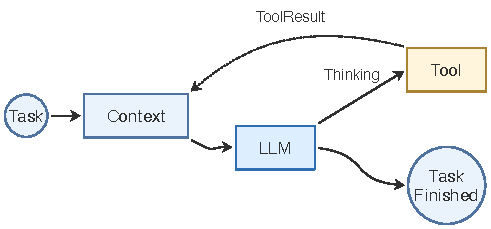
\includegraphics[width=0.98\columnwidth]{images/Motivation/agentic_tool_loop.pdf}
    \vspace{-0.2in}
    \caption{Workflow of an LLM agent.}
    \label{fig:workflow}
    \vspace{-0.2in}
\end{figure}




LLM-powered agents are becoming a common execution model for long-running tasks such as deep research, software debugging, and scientific analysis~\cite{adminKimiResearcherKimi2025, GeminiCLIBuild2025, ClaudeCodeClaude, GitHubCopilotYour2025, claudeskills}. As exemplified by OpenAI Deep Research~\cite{IntroducingDeepResearch2025} and Manus~\cite{ManusHandsAI}, the LLM acts as the ``brain'' of the agent: it decomposes a complex task into sub-steps and invokes external tools to interact with the outside world~\cite{luo2025autellix, zhang2026megaflow, giusti2025federation}.

A modern LLM-powered agent follows an \emph{Iterative LLM--Tool Loop}, as shown in Fig.~\ref{fig:workflow}. \v2{Agent execution is semantically sequential: each step depends on the output of the previous step. In today's agent systems like Codex and Qwen Code, however, this semantic order is typically realized as a physically serialized path: the LLM generates, emits a tool call, waits for the tool result, and then resumes generation.} As a result, LLM generation and tool execution form a single critical path. Therefore, the agent serving system's latency objective shifts from minimizing token-level latency to minimizing task-level end-to-end (E2E) latency.

This execution model makes task-level E2E latency the central objective for agent serving, and exposed tool time a task-level bottleneck. Two observations motivate our work:

First, tool execution is a major part of the critical path: in our measurements (\S\ref{sec:inefficiencies}; Fig.~\ref{fig:moti:single}), it accounts for 45\%--57\% of agent E2E latency across representative deep research, coding, and scientific tasks. Because this tool portion lies on the serialized critical path, reducing task E2E latency requires reducing the exposed tool time, not just accelerating LLM generation. To move tool execution earlier without changing semantic order, the system must know concrete future tool invocations before they appear on the serialized path. 

Second, future tool use is often predictable before the LLM explicitly emits the next tool call. As Fig.~\ref{fig:motifs} shows, real traces show recurring sub-workflow patterns, such as \textit{search} followed by \textit{visit}, \textit{edit} followed by \textit{run test}, \textit{grep} followed by \textit{file\_editor}. These patterns often carry implicit data dependencies, where subsequent tool call's inputs are already contained in earlier calls' outputs. For example, 55\% of successful \textit{file\_editor} calls are followed by terminal execution, and in 95\% of web visits the URL is a strict substring of the preceding search output (\S\ref{subsec:opportunities}). \v2{Therefore, future tool invocations can often be predicted before they appear on the serialized path.}

\begin{figure}[t]
    \centering
    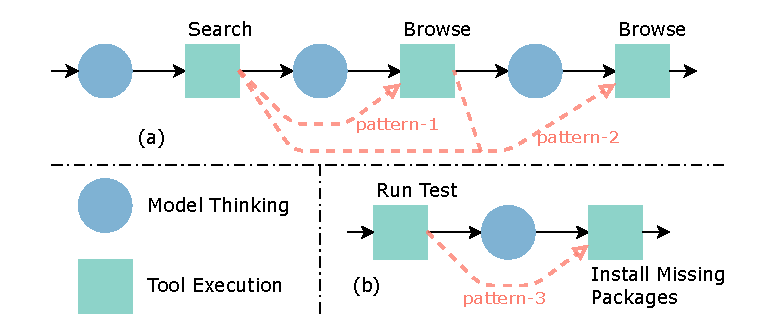
\includegraphics[width=\linewidth]{images/examples/motifs.pdf}
    \vspace{-0.15in}
    \caption{Example recurring tool-call patterns and latent data dependencies in agent traces.}
    \label{fig:motifs}
    \vspace{-0.15in}
\end{figure}

\v2{Together, these two observations create an opportunity for serving-level parallelization: the system can reduce substantial exposed tool time by predicting concrete future tool invocations and executing them while the LLM is still generating. Instead of waiting for the LLM to emit every tool call, we can execute these invocations speculatively. This speculative execution creates temporal overlap between the tool execution and LLM generation. Through this overlap, the serving system parallelizes tool execution and LLM generation without changing the agent's semantically sequential workflow.}

However, to fully take advantage of this opportunity, we must address two challenges. First, effective speculation must predict concrete future invocations under uncertainty, not only tool names. The same pattern can imply different arguments in different sessions, and wrong arguments waste speculative work because the speculative results are not reusable when the authoritative invocation arrives. \v2{Second, blind speculation can create LLM--tool phase imbalance. Uncoordinated parallelization does not always reduce task-level latency:} correct speculation \v2{shortens exposed tool time, but it can also make many sessions become ready for LLM generation earlier and closer together, shifting the bottleneck from the tool phase to the LLM phase.} \v2{Because LLM generation is load-sensitive (\S\ref{subsec:observation2}), this phase imbalance could increase decoding time or queueing and erase the tool-side gain. On the other hand, inaccurate speculation further creates speculative results the LLM never consumes.} The system must jointly decide when to execute speculative tool calls and how to pace sessions that return from tool-side into the LLM batch, avoiding phase imbalance that converts tool acceleration into LLM slowdown.

Existing LLM-serving and agentic-serving systems are tool-unaware and therefore do not address the above challenges. General LLM serving systems are organized around token-level serving efficiency and schedule ready LLM requests as the primary workload~\cite{kwon2023efficient, agrawal2024sarathiserve, duan2024muxserve, qiao2024conserve}. Agentic-serving systems add session-aware mechanisms, but still treat a tool call as an external waiting interval between two LLM requests~\cite{abhyankar2024infercept, wang2025augserve, pan2025kvflow, xie2025strata, li2025throughput}. As a result, \v2{these systems cannot jointly optimize tool execution and LLM generation.} Because tool execution sits outside their scheduling loop, they leave tool time exposed on the task critical path; because they lack visibility into tool returns, they cannot pace sessions before they re-enter the LLM engine. Even if another mechanism shortens tool latency, the saved time can reappear as bursty LLM arrivals that push the GPU away from its latency-efficient region.



% To address these challenges, we propose \textbf{P}attern-\textbf{A}ware \textbf{S}peculative \textbf{T}ool \textbf{E}xecution (\textbf{\sys}), \v2{a coordinated tool-LLM parallelization system.} Figure~\ref{fig:overlap-paradigm} contrasts an uncoordinated agentic serving system and \sys: the baseline runs LLM generation and tool execution without coordination, so the LLM batch size oscillates between under-utilization and overload, while \sys overlaps tool execution with LLM generation and paces returning sessions so that the LLM batch size stays inside the optimal region.

To address these challenges, we propose \textbf{P}attern-\textbf{A}ware \textbf{S}peculative \textbf{T}ool \textbf{E}xecution (\textbf{\sys}), a coordinated tool--LLM parallelization system for agent serving. \sys exploits recurring agent patterns to move concrete tool execution earlier in physical time, while preserving the agent's semantically sequential execution. Instead of treating the LLM engine and tool executor as independent components, \sys places a control plane across both phases: it speculates on likely future tool calls, isolates speculative results until they are confirmed by the LLM, and controls when completed sessions re-enter the LLM engine.

% \sys has two core components. First, the Pattern Analyzer predicts future tool invocations based on recurring agent patterns. \sys then executes these predicted calls speculatively while the LLM generates the authoritative tool-call decision, thereby overlapping tool execution with ongoing LLM generation. Second, the Online Scheduler jointly manages authoritative invocations, speculative invocations, and returning LLM generations. Using tool-side and LLM-side state, it decides when to run speculative work and how to pace returning sessions, keeping active LLM load away from both under-utilization and overload so that \v2{serving-level parallelization translates into} task E2E speedup.

\sys consists of three core components: the Pattern Analyzer, the Tool Speculation Scheduler, and the LLM--Tool Co-Scheduler. The Pattern Analyzer mines recurring control flow and implicit data flow from prior agent traces, then instantiates concrete future tool invocations from live session state. The Tool Speculation Scheduler coordinates authoritative and speculative invocations. It admits speculative work when it is likely to hide exposed tool time, isolates speculative results until confirmation, and preserves priority for authoritative tool calls. The LLM--Tool Co-Scheduler paces returning sessions to keep the LLM engine away from both under-utilization and overload. Together, these components turn predictable tool waits into effective overlap with LLM generation, yielding task-level end-to-end speedup without changing agent semantics.

We implement \sys as a full-stack system spanning agent applications and the vLLM serving stack, covering both tool-side execution and LLM-side scheduling. Our evaluation demonstrates that compared to state-of-the-art baselines, \sys reduces the average task completion time by 43.5\% and speeds up average tool execution by 1.8$\times$.

The main contributions of this paper are as follows:

\begin{itemize}[itemsep=0pt, parsep=2pt, labelsep=5pt, leftmargin=*, topsep=2pt,partopsep=2pt]
\item \textbf{Characterization of the LLM--tool critical path.} We show that tool execution is a major critical-path component, and future tool invocations can often be predicted before they appear on the serialized path.
\item \textbf{Coordinated tool--LLM parallelization.} We propose \sys, which combines the Pattern Analyzer, the Tool Speculation Scheduler, and the LLM--Tool Co-Scheduler to turn recurring agent patterns into concrete predictions, execute speculative tool calls without interfering with authoritative execution, and preserve tool-side gains through LLM-side pacing.
\item \textbf{Full-stack implementation and evaluation.} We implement \sys across agent applications and the vLLM serving stack; compared to state-of-the-art baselines, \sys reduces the average task completion time by 43.5\% and speeds up average tool execution by 1.8$\times$.
\end{itemize}
